\documentclass{article}

%
% 引入模板的style文件
%
\usepackage{homework}

\setCJKmainfont{SimSun}[AutoFakeBold] %宋体加粗
\setCJKsansfont{SimHei}[AutoFakeBold] %黑体加粗


\usepackage{minted} %配合minted宏包进行好看的高亮
\usepackage{currfile} %配合minted宏包进行好看的高亮
\usepackage{caption} %配合minted宏包进行好看的高亮
\usepackage{tcolorbox} %配合minted宏包进行好看的高亮
\usepackage{xcolor} %配合minted宏包进行好看的高亮
\tcbuselibrary{skins} %配合minted宏包进行好看的高亮
\tcbuselibrary{minted} %配合minted宏包进行好看的高亮
\usemintedstyle{paraiso-dark} %配合minted宏包进行好看的高亮
\usepackage{framed} 
\usepackage{amsmath}


%
% 封面
%


\title{
	
\includegraphics[width=0.6\textwidth]{images/title/ucas_logo 1.pdf}\\
    \vspace{1in}
    \textmd{\textbf{\hmwkClass}}\\
	\textmd{\Large{\textbf{\hmwkClassID}}}\\
    \textmd{\textbf{\hmwkTitle}}\\
    \normalsize\vspace{0.1in}\large{\hmwkCompleteTime }\\
    \vspace{0.1in}\large{\textit{\hmwkClassInstructor\ }}\\
    \vspace{1in}
	
\includegraphics[width=0.25\textwidth]{images/title/Cyber.jpg}\\
	\vspace{1in}
}

\author{
	\hmwkAuthorName \\ 
	\hmwkAuthorStuID \\
	\hmwkAuthorInst \\
	\hmwkAuthorzhuanye \\
	\hmwkAuthorfangxiang
	}
\date{}

\renewcommand{\part}[1]{\textbf{\large Part \Alph{partCounter}}\stepcounter{partCounter}\\}


%
% 正文部分
%
\begin{document}


\maketitle


%\include{chapters/ch01}
%\include{chapters/ch02}
%\include{chapters/ch03}
%\include{chapters/ch04}
%\include{chapters/ch05}


\pagebreak



\begin{homeworkProblem}
	最大子段和问题: 给定整数序列$a_1, a_2, \cdots, a_n$, 求该序列形如$\displaystyle \sum_{k=i}^j a_k$的子段和的最大值: $$\displaystyle \text{max} \left\{0, \underset{1\le i\le i\le n}{\text{max}} \sum_{k=i}^j a_k\right\}$$
	
	(1). 已知一个简单算法如下:
\begin{tcblisting}{listing engine=minted,boxrule=0.1mm,
colback=blue!5!white,colframe=blue!75!black,
listing only,left=5mm,enhanced,sharp corners=all,
overlay={\begin{tcbclipinterior}\fill[red!20!blue!20!white] (frame.south west)
rectangle ([xshift=5mm]frame.north west);\end{tcbclipinterior}},
minted language=c++,
minted style=tango,
minted options={fontsize=\small,breaklines,autogobble,linenos,numbersep=3mm}}
int Maxsum(int n, vector<int> a, int& besti, int& bestj) {
    int sum = 0;
    for(int i = 1; i <= n; i++) {
        int suma = 0;
        for(int j = i; j <= n; j++) {
            suma += a[j];
            if(suma > sum) {
                sum = suma;
                besti = i;
                bestj = j;
            }
        }
    }
    return sum;
}
\end{tcblisting}
	试分析该算法的时间复杂性;

	(2). 试用分治算法解最大子段和问题, 并分析算法的时间复杂性;

	(3). 试说明最大子段和问题具有最优子结构性质, 并设计一个动态规划算法求解最大子段和问题, 分析算法的时间复杂度. (提示: 可令$\displaystyle b\left( j \right) =\underset{1\le i\le j\le n}{\text{max}}\sum_{k=i}^j{a_k}, j=1,2,\cdots ,n$)
	\\

	\solution \,\,(1). 显然第2层for循环里面的操作都是常数次的(记为$C$), 所以算法总的关键操作数为$$\sum_{i=1}^n{\sum_{j=i}^n{C}}=C\sum_{i=1}^n{\left( n-i+1 \right)}=\frac{1}{2}C\left( n^2+n \right) 
	$$
	故显然时间复杂度为$T(n)=O(n^2)$.

	(2). 采用分治算法, 则考虑: 先将数组从中间mid切开. 此时, 最大和的子段可能出现在左半边, 也可能出现在右半边, 也有可能横跨左右两个子数组. 所以需要返回这三种情况下所分别对应的子问题解的最大值. 

	当最大和的子段出现在左半边(右半边同理)时, 继续分中点递归直至分解到只有一个数为止;

	当最大和的子段横跨mid左右时, 只需分别求解左子数组的最优后缀和以及右子数组的最优前缀和. 这三种情形下的最大值即为整个数组的最大子段和. 具体分治算法的C++代码见后页. 从C++代码可以看出最坏情形下的时间复杂度的递推式和结果分别为$$T\left( n \right) =2T\left( \frac{n}{2} \right) +O\left( \frac{n}{2} \right) +O\left( \frac{n}{2} \right) =2T\left( \frac{n}{2} \right) +O\left( n \right)
	$$
	故根据主定理($\log_b(a)=\log_2(2)=1=d$)可知$T(n)=O(n\log n)$.
\begin{tcblisting}{listing engine=minted,boxrule=0.1mm,
colback=blue!5!white,colframe=blue!75!black,
listing only,left=5mm,enhanced,sharp corners=all,
overlay={\begin{tcbclipinterior}\fill[red!20!blue!20!white] (frame.south west)
rectangle ([xshift=5mm]frame.north west);\end{tcbclipinterior}},
minted language=c++,
minted style=tango,
minted options={fontsize=\small,breaklines,autogobble,linenos,numbersep=3mm}}
class Solution {
public:
    int maxSubArray(vector<int>& nums) {
        return maxSum(nums, 0, nums.size() - 1);
    }

    int maxSum(vector<int> nums, int left, int right) {
        if(left == right) {
            return nums[left];
        }
        int mid = (left + right) >> 1;
        int LeftRes = maxSum(nums, left, mid);  //可能情况1
        int RightRes = maxSum(nums, mid + 1, right);  //可能情况2
        /*可能情况3: 最大(和)子段出现横跨mid(切分点)两边*/
        int lbs = INT_MIN, sum1 = 0;
        for(int i = mid; i >= left; i--) { //一次向前扫描来求得最大后缀和
            sum1 += nums[i];
            if(sum1 > lbs) {
                lbs = sum1;
            }
        }
        int rbs = INT_MIN, sum2 = 0;
        for(int i = mid + 1; i <= right; i++) { //一次向后扫描来求得最大前缀和
            sum2 += nums[i];
            if(sum2 > rbs) {
                rbs = sum2;
            }
        }
        return max(LeftRes, max(RightRes, lbs + rbs)); //返回三种情形下的最大值
    }
};
\end{tcblisting}
	(3). 先证明此问题具有最优子结构性质: 依次考虑($1\leq i\leq n$)以$a[i]$\textbf{为结尾}的最大子段和$C[i]$, 然后在这$n$个值当中取最大值即为原问题答案. 假设以$a[i]$为结尾的最大(和)子段为$\{a[k],\cdots,a[i]\}$, 那么$\{a[k],\cdots,a[i-1]\}$一定是以$a[i-1]$为结尾的最大(和)子段. 否则若$\{a[m],\cdots,a[i-1]\}$为以$a[i-1]$为结尾的最大(和)子段, 那么$\{a[m],\cdots,a[i-1],a[i]\}$就是以$a[i]$为结尾的最大(和)子段, 这显然与假设相矛盾, 也就是说该优化函数是满足优化原则的(即此问题具有最优子结构性质). 

	现在来推导$C[i]$的递推表达式: 当$C[i-1]\leq 0$, 说明$C[i-1]$对应的子段对于整体的贡献是没有的, 所以$C[i]\gets a[i]$; 当$C[i-1]>0$, 说明$C[i-1]$对应的子段对于整体的是有贡献的, 于是$C[i]\gets a[i]+C[i-1]$. 两种可能情况(对应两种决策)取最大值即可:$$\begin{cases}
		C\left[ i \right] =\text{max} \left\{ a\left[ i \right] ,C\left[ i-1 \right] +a\left[ i \right] \right\} , 2\le i\le n\\
		C\left[ 1 \right] =a\left[ 1 \right]\\
	\end{cases}
	$$
	最后返回数组$C$中的最大值($\displaystyle \underset{1\le i\le n}{\text{max}}C\left[ i \right] $)即可. 计算$C[i]$的过程需要消耗$O(n)$的时间, 找出数组最大值也需要$O(n)$的时间(一次遍历), 所以算法的总时间复杂度为$T(n)=O(n)$. 并且我们可以给出后页的C++代码:
\begin{tcblisting}{listing engine=minted,boxrule=0.1mm,
colback=blue!5!white,colframe=blue!75!black,
listing only,left=5mm,enhanced,sharp corners=all,
overlay={\begin{tcbclipinterior}\fill[red!20!blue!20!white] (frame.south west)
rectangle ([xshift=5mm]frame.north west);\end{tcbclipinterior}},
minted language=c++,
minted style=tango,
minted options={fontsize=\small,breaklines,autogobble,linenos,numbersep=3mm}}
#include <algorithm>
#include <iostream>
#include <vector>
#include <limits.h>
using namespace std;

int mostvalue(vector<int>& a) { //时间复杂度为O(n), 空间复杂度为O(n)
    int n = a.size();
    vector<int> dp(n);
    dp[0] = a[0];
    for(int i = 1; i < n; i++) {
        dp[i] = max(dp[i - 1] + a[i], a[i]);
    }
    int index = max_element(dp.begin(), dp.end()) - dp.begin();
    return dp[index];
}

int mostvalue2(vector<int>& a) {  //时间复杂度为O(n), 空间复杂度为O(1)
    int n = a.size();
    int dp = a[0];
    int res = INT_MIN;
    for(int i = 1; i < n; i++) {
        dp = max(dp + a[i], a[i]);  //使用滚动数组思想来优化空间
        res = max(res, dp); //迭代式更新求得最大值
    }
    return res;
}

int main() {
    int N;
    scanf("%d", &N);
    vector<int> a(N);
    for(int i = 0; i < N; i++){
        scanf("%d", &a[i]);
    }
    //int res = mostvalue(a); //不优化空间
    int res = mostvalue2(a); //优化空间
    cout << res;
    
}
\end{tcblisting}
\end{homeworkProblem}


\pagebreak

\begin{homeworkProblem}
	设$A=\left\{ x_1,x_2,\cdots ,x_n \right\} $是$n$个不等的整数构成的序列, $A$的一个单调递增子序列是指序列$\{ x_{i_1},x_{i_2},$
	$\cdots ,x_{i_k} \} ,i_1<i_2<\cdots i_k	$且$x_{i_1}<x_{i_2}<\cdots <x_{i_k}$.(子序列包含$k$个整数). 例如, $A=\left\{ 1,5,3,8,10,6,4,9 \right\} $, 他的长度为4的递增子序列是: $\left\{ 1,5,8,10 \right\} ,\left\{ 1,5,8,9 \right\} ,\cdots$.设计一个算法, 求$A$的最长的单调递增子序列, 分析算法的时间复杂度. 对于输入实例$A=\left\{ 2,8,4,-4,5,9,11 \right\} $, 给出算法的计算过程和最后的解.
	\\

	\solution 定义$dp[i]$是以$\text{nums}[i]$\textbf{为结尾}(且考虑前$i$个元素)的最长单增子序列的长度. 
    \begin{itemize}
        \item 如果在索引范围$[0,i-1]$当中能够找到(若干个)下标$j$使得$\text{nums}[j]<\text{nums}[i]$成立. 根据\textbf{大小关系的传递性}可知: 以$\text{nums}[j]$为结尾的最长递增子序列中的所有元素都$<\text{nums}[i]$, 也就是说我们找到了符合条件的位置. 那么在这些位置$j$中找到$dp[j]$的最大值, 在此基础上加1即可使得以$\text{nums}[i]$为结尾的单增子序列长度最大(即将nums$[i]$接到符合条件的、且最长的nums$[j]$后边).
        \item 如果在索引范围$[0,i-1]$当中找不到下标$j$使得$\text{nums}[j]<\text{nums}[i]$成立(即$\text{nums}[0,\cdots,i-1]$都比$\text{nums}[i]$大), 那么以nums$[i]$为结尾的单增子序列长度就只能为1(即nums$[i]$独立作为单增子序列).
    \end{itemize}

    故综合上述两种情况, 我们可以写出如下转移方程$(i\geq 1)$和初始条件:
    $$
    dp\left[ i \right] =\left\{ \begin{matrix}
        \underset{0\le j\le i-1}{\text{max}}dp\left[ j \right] +1,&		\exists j\in \left[ 0,i-1 \right] , s.t. \,\text{nums}\left[ j \right] <\text{nums}\left[ i \right]\\
        1&		\forall j\in \left[ 0,i-1 \right] , s.t. \,\text{nums}\left[ j \right] >\text{nums}\left[ i \right]\\
    \end{matrix} \right. , dp\left[ 0 \right] =1
    $$

    但是上述递推方程只能给出长度, 并不能给出具体的最优解, 所以我们需要借助一个数组$m$来对解进行回溯\footnote{对于求\textbf{具体方案}的动态规划题目, 多开一个数组来记录状态的转移情况是\textbf{最常见}的手段.}(即$m[i]$记录$dp[i]$是由哪个下标的状态转移而来的). 而要想算出\textbf{整个数组}的最长单增子序列长度, 则需要算好所有的$dp[i]$值, 再对$dp$数组进行遍历, 由此得到最长单增子序列长度和对应下标\footnote{因为整个数组的最长单增子序列\textbf{不一定}以nums$[n-1]$为结尾! 故才需要求得$dp$数组的最大值.}. 最后使用数组$m$进行回溯以取得答案. 可以看出, 算法的空间复杂度为$O(n)$, 而时间复杂度显然为$$T\left( n \right) =O\left( \sum_{i=0}^{n-1}{\sum_{j=0}^{i-1}{1}} \right) =O\left( \sum_{i=0}^{n-1}{i} \right) =O\left( \frac{n\left( n-1 \right)}{2} \right) =O\left( n^2 \right) 
	$$
	对于具体实例, 计算过程如下:
	\begin{align}
		&C\left[ 1 \right] =1; C\left[ 2 \right] =2,k\left[ 2 \right] =1; C\left[ 3 \right] =2,k\left[ 3 \right] =1; C\left[ 4 \right] =1,k\left[ 4 \right] =0; \notag
		\\
		&C\left[ 5 \right] =3, k\left[ 5 \right] =3; C\left[ 6 \right] =4,k\left[ 6 \right] =5; C\left[ 7 \right] =5,k\left[ 7 \right] =6 \notag
	\end{align}
	显然在数组$C$中的最大值为$C[7]=5$, 即最长递增子序列长度为5且追踪过程为: $$x_7,k\left[ 7 \right] =6\Rightarrow x_6;\,\, k\left[ 6 \right] =5\Rightarrow x_5;\,\, k\left[ 5 \right] =3\Rightarrow x_3;\,\, k\left[ 3 \right] =1\Rightarrow x_1
	$$
	故$A=\left\{ 2,8,4,-4,5,9,11 \right\} $的最长单调递增子序列为$\left\{ x_1,x_3,x_5,x_6,x_7 \right\} =\left\{ 2,4,5,9,11 \right\}$.

	我们将上述的最优值求解过程和解的回溯过程写成C++代码, 并且已完全通过\href{https://leetcode.cn/problems/longest-increasing-subsequence/description/}{\textbf{LeetCode-T300}}的所有测试样例, 具体如后页所示:
	\newpage
\begin{tcblisting}{listing engine=minted,boxrule=0.1mm,
colback=blue!5!white,colframe=blue!75!black,
listing only,left=5mm,enhanced,sharp corners=all,
overlay={\begin{tcbclipinterior}\fill[red!20!blue!20!white] (frame.south west)
rectangle ([xshift=5mm]frame.north west);\end{tcbclipinterior}},
minted language=c++,
minted style=tango,
minted options={fontsize=\small,breaklines,autogobble,linenos,numbersep=3mm}}
#include <algorithm>
#include <ctime>
#include <iostream>
#include <vector>
using namespace std;
vector<int> LIS(vector<int>& nums) {
    int n = nums.size();
    vector<int> dp(n, 0);
    dp[0] = 1;
    vector<int> m(n, 0); // m[0] = 0
    for (int i = 1; i <= n - 1; i++) {
        int prev = i, len = 1; //至少包含自身一个数, 因此起始长度为1, 由自身转移而来
        for (int j = 0; j <= i - 1; j++) {
            if (nums[j] < nums[i]) { //找到满足条件的位置j
                if (dp[j] + 1 > len) {
                    len = dp[j] + 1;
                    prev = j; //迭代式更新求得满足条件的d[j]+1的最大值和dp[i]的来源(即prev)
                }
            }
        }
        dp[i] = len, m[i] = prev; // m[i]就是nums[i]的来源位置(即prev)!
    }
    int index = max_element(dp.begin(), dp.end()) - dp.begin(); //最大值对应的索引
    int MaxLen = dp[index]; //递增子序列的最大长度值
    vector<int> res; //注意整个数组的最长递增子序列是以nums[index]为结尾的!
    while (res.size() != MaxLen) {
        res.push_back(nums[index]);
        index = m[index]; //逐步地从后往前回溯索引, 并将对应元素写进res数组
    }
    reverse(res.begin(), res.end()); //reverse一下更好看一些, 此步可以选择注释掉
    return res;
}
int main() {
    int n;
    cin >> n;            //输入数组的长度
    vector<int> nums(n); //定义数组
    cout << "数组nums为:" << endl;
    for (int i = 0; i < n; i++) { //对数组初始化
        nums[i] = -1 * (n + 1) +
                  rand() % (2 * n + 2); //在[-n - 1, n + 1]随机产生长度为n的数组
        cout << nums[i] << " "; //打印该数组
    }
    cout << endl;
    clock_t startTime = clock(); //计时开始
    vector<int> res = LIS(nums);
    clock_t endTime = clock(); //计时结束
    cout << "数组nums的最长单增子序列为:" << endl;
    for (int i = 0; i < res.size(); i++) {
        cout << res[i] << " ";
    }
    cout << endl;
    cout << "算法耗时为: " << (double)(endTime - startTime) << "ms" << endl;
}
\end{tcblisting}
	在解决这个问题之后, 我们需要再给出另一个解决思路与此非常类似的问题以便进行类比学习: \textbf{最大整除子集问题}: 给定一组互异的正整数集合, 找到最大子集: 使得子集元素中的每一对$(S_i,S_j)$都满足$S_i\%S_j=0$或$S_j\% S_i=0$. 请返回最大子集的阶数(即子集中的元素个数). \textbf{注意}: $S_i\%S_j=0$意味着$S_i$可以被$S_j$整除.

	由于整除子集中的每一对值都是倍数\textbf{或}约数关系, 因此为了后续解决问题的方便, 我们不妨先将数组nums进行排序(耗时为$O(n\log n)$, (后续可知)不影响整个算法的复杂度), 以免还要具体考虑一对值\textbf{到底是}倍数关系还是约数关系(思考起来会很乱), 并且对nums排好序有助于我们利用\textbf{整除关系的传递性}来进行动态规划! 
    
    于是我们定义: $dp[i]$是以$\text{nums}[i]$\textbf{为结尾}(且考虑前$i$个元素)的最大整除子集的阶数(即该子集合的元素个数).
    \begin{itemize}
        \item 如果在索引范围$[0,i-1]$当中能够找到(若干个)下标$j$使得$\text{nums}[i] \% \text{nums}[j]\text{==}0$成立. 由于$\text{nums}[j]\,|\,\text{nums}[i]$且根据\textbf{整除关系的传递性}可知: 以$\text{nums}[j]$为结尾的最大整除子集中的所有元素都能整除$\text{nums}[i]$, 也就是说我们找到了符合条件的位置. 那么在这些位置$j$中找到$dp[j]$的最大值, 在此基础上加1即可使得以$\text{nums}[i]$为结尾的整除子集的长度最大(即将nums$[i]$接到符合条件的、且最长的nums$[j]$后边).
        \item 如果在索引范围$[0,i-1]$当中找不到下标$j$使得$\text{nums}[i] \% \text{nums}[j]\neq 0$成立(即$\text{nums}[i]$不能接在位置$i$之前的任何数的后面!), 那么以nums$[i]$为结尾的最大整除子集的长度就只能为1(即nums$[i]$独立作为最大整除子集).
    \end{itemize}
    故综合上述两种情况, 我们可以写出如下转移方程$(i\geq 1)$和初始条件:
    $$
    dp\left[ i \right] =\left\{ \begin{matrix}
        \underset{0\le j\le i-1}{\text{max}}dp\left[ j \right] +1,&		\exists j\in \left[ 0,i-1 \right] , s.t.\, \text{nums}\left[ i \right] \%\text{nums}\left[ j \right] =0\\
        1&		\forall j\in \left[ 0,i-1 \right] , s.t. \,\text{nums}\left[ i \right] \%\text{nums}\left[ j \right] \ne 0\\
    \end{matrix} \right. , dp\left[ 0 \right] =1
    $$
    此时我们需要借助一个数组$m$来对解进行回溯(即$m[i]$记录$dp[i]$是由哪个下标的状态转移而来的). 而要想算出\textbf{整个数组}的整除子集的最大长度, 则需要算好所有的$dp[i]$值, 再对$dp$数组进行遍历, 由此得到最大的整除子集长度和对应下标. 最后使用数组$m$进行回溯以取得答案. 于是我们可以给出最大整除子集算法的C++代码:
\begin{tcblisting}{listing engine=minted,boxrule=0.1mm,
colback=blue!5!white,colframe=blue!75!black,
listing only,left=5mm,enhanced,sharp corners=all,
overlay={\begin{tcbclipinterior}\fill[red!20!blue!20!white] (frame.south west)
rectangle ([xshift=5mm]frame.north west);\end{tcbclipinterior}},
minted language=c++,
minted style=tango,
minted options={fontsize=\small,breaklines,autogobble,linenos,numbersep=3mm}}
class Solution {
public:
    vector<int> largestDivisibleSubset(vector<int>& nums) {
        sort(nums.begin(), nums.end());  //先对数组进行排序, 方便后续考虑递推表达式
        int n = nums.size();
        vector<int> dp(n, 0);
        dp[0] = 1;
        vector<int> m(n, 0); // m[0] = 0
        for (int i = 1; i <= n - 1; i++) {
            int prev = i, len = 1; //至少包含自身一个数, 因此起始长度为1, 由自身转移而来
            for (int j = 0; j <= i - 1; j++) {
                if (nums[i] % nums[j] == 0) {
                    if (dp[j] + 1 > len) {
                        len = dp[j] + 1;
                        prev = j; //迭代式更新求得满足条件的d[j]+1的最大值和dp[i]的来源(即prev)
                    }
                }
            }
            dp[i] = len, m[i] = prev; // m[i]就是nums[i]的来源位置(即prev)!
        }
\end{tcblisting}
\begin{tcblisting}{listing engine=minted,boxrule=0.1mm,
colback=blue!5!white,colframe=blue!75!black,
listing only,left=5mm,enhanced,sharp corners=all,
overlay={\begin{tcbclipinterior}\fill[red!20!blue!20!white] (frame.south west)
rectangle ([xshift=5mm]frame.north west);\end{tcbclipinterior}},
minted language=c++,
minted style=tango,
minted options={fontsize=\small,breaklines,autogobble,linenos,numbersep=3mm}}
        int index = max_element(dp.begin(), dp.end()) - dp.begin(); //最大值对应的索引
        int MaxLen = dp[index]; //整除子集的最大长度值
        vector<int> res; //注意整个数组的最大整除子集是以nums[index]为结尾的!
        while (res.size() != MaxLen) {
            res.push_back(nums[index]);
            index = m[index]; //逐步地从后往前回溯索引, 并将对应元素写进res数组
        }
        reverse(res.begin(), res.end()); //reverse一下更好看一些, 此步可以选择注释掉
        return res;
    }
};
\end{tcblisting}
	上述C++代码已完全通过\href{https://leetcode.cn/problems/largest-divisible-subset/description/}{\textbf{LeetCode-T368}}的所有测试样例. 再来分析一下该算法的时空复杂度: 排序需要$O(n\log n)$的时间, 算法主体显然需要消耗$O(n^2)$的时间, 而其余操作(如reverse操作、求dp最大值以及结果写入)均只需要$O(n)$的时间, 所以综合可得算法的时间复杂度为$O(n^2)$. 由于借助了两个长度为$n$的中间数组, 所以算法的空间复杂度为$O(n)$. 上述两个算法之所以正确, 本质上是利用了\textbf{二元关系的可传递性}. 比如最长递增子序列是利用了\textbf{大小关系“$>$”的可传递性}, 而最大整除子集利用了\textbf{整除关系“$\mid$”的可传递性}. 这两段代码基本一样, 所以可以将此记住作为解题模板, 以便应付其他具有传递性的二元关系的dp算法题.
\end{homeworkProblem}

\begin{homeworkProblem}
	考虑下面特殊的整数线性规划问题
	$$
	\begin{array}{l}
		\displaystyle \text{max}  \sum_{i=1}^n{c_ix_i}\\
		\displaystyle \sum_{i=1}^n{a_ix_i\le b, x_i\in \left\{ 0,1,2 \right\} ,1\le i\le n}\\
	\end{array}
	$$
	试设计一个解决此问题的动态规划算法, 并分析算法的时间复杂度.
	
	\solution \textbf{方法1}: 设$y_i\in \left\{ 0,1 \right\} ,1\le i\le 2n,$ 令$x_i=y_i+y_{i+n},1\leq i \leq n$, 则上述规划问题转化为
	$$
	\begin{array}{l}
		\displaystyle \text{max}  \sum_{i=1}^{2n}{c_iy_i}\\
		\displaystyle \sum_{i=1}^{2n}{a_iy_i\le b, y_i\in \left\{ 0,1 \right\} ,1\le i\le 2n}\\
	\end{array}
	$$
	其中$c_{i+n}=c_i,a_{i+n}=a_i,1\leq i \leq n$. 将$c_i$看作价值, $a_i$看作重量, $b$看作背包容量. 于是就将问题转化为了0-1背包问题(物品数为$2n$). 由于$n$件物品的0-1背包问题的动态规划算法的时间复杂度为$O\left( 2^n \right)$, 故此方法的时间复杂度为$O\left( 2^{2n} \right) =O\left( 4^n \right) $.

	\textbf{方法2}: 可以看成是另一种背包问题. 即$b$为背包容量, $x_i\in \left\{ 0,1,2 \right\}$为背包中可以装0,1或者2件物品, $x_i$对应的价值为$c_i$, 求在容量$b$一定的前提下, 背包所容纳物品的最大价值. 也就是参数完全相同的两个0-1背包问题, 它们同时制约于背包容量为$C$这个条件.

	在设计算法时可以优先考虑$m_i$, 也就是先判断背包剩下的容量能不能放进去$c_i$, 若可以就再判断能否使$p_i=1$, 若可以那就再放入一个$c_i$, 这样就间接地满足了$x_i=m_i+p_i=2$的条件. 根据单参数的0-1背包问题的动态规划算法, 于是可以类比写出该问题的递推公式
	$$
	m\left(k,x\right)=\begin{cases}
		-\infty,&		x<0\\
		m\left( k-1,x \right),&		0\le x<w_k\\
		\text{max} \left\{ m\left( k-1,x \right) ,m\left( k-1,x-w_k \right) +p_k \right\},&		w_k\le x<2w_k\\
		\text{max} \left\{ m\left( k-1,x \right) ,m\left( k-1,x-w_k \right) +p_k,m\left( k-1,x-2w_k \right) +2p_k \right\},&		x\ge 2w_k\\
	\end{cases}
	$$
	类似讲义中的推导过程可以得出该方法的时间复杂度为$O\left( 3^n \right)$.
\end{homeworkProblem}

\begin{homeworkProblem}
	可靠性设计: 一个系统由$n$级设备串联而成, 为了增强可靠性, 每级都可能并联了不止一台同样的设备. 假设第$i $级设备$D_i$用了$m_i$台, 该级设备的可靠性$g_i(m_i)$, 则这个系统的可靠性是$\Pi g_i(m_i)$. 一般来说$g_i(m_i)$都是递增函数, 所以每级用的设备越多系统的可靠性越高. 但是设备都是有成本的, 假定设备$D_i$的成本是$c_i$, 设计该系统允许的投资不超过$c$. 那么, 该如何设计该系统(即各级采用多少设备)使得这个系统的可靠性最高. 试设计一个动态规划算法求解可靠性设计问题.

	\solution 问题描述为
	$$
	\begin{array}{l}
		\displaystyle \text{max}  \,\prod_{i=1}^n{g_i\left( m_i \right)}\\
		\displaystyle \text{s}.\text{t}.\, \sum_{i=1}^n{m_ic_i\le c, 1\le m_i\le 1+ \left\lfloor \frac{c-\sum_{i=1}^n{c_i}}{c_n}\right\rfloor }\\
	\end{array}
	$$
	记$G[k](x)$为第$k$级设备在可用投资为$x$时的系统可靠性最大值则有如下关系式$$
	G\left[ k \right] \left( x \right) =\underset{1\le m_k\le \left\lfloor \frac{x}{c_k} \right\rfloor}{\text{max}}\left\{ g_k\left( m_k \right) \cdot G\left[ k-1 \right] \left( x-c_km_k \right) \right\} 
	$$
	定义下列函数
	$$
	G\left[ k \right] \left( x \right) =\begin{cases}
		-\infty ,&		\displaystyle x<\sum_{i=k}^n{c_i}\\
		\underset{1\le m_k\le \text{min} \left\{ \left\lfloor \frac{x}{c_1} \right\rfloor ,\left\lfloor \frac{c}{c_k} \right\rfloor \right\}}{\text{max}}\left\{ g_k\left( m_k \right) \cdot G\left[ k-1 \right] \left( x-c_km_k \right) \right\} ,&		\displaystyle x\ge \sum_{i=k}^n{c_i}\\
	\end{cases}
	$$
	$$
	G\left[ 0 \right] \left( x \right) =\left\{ \begin{matrix}
		1,&		\displaystyle \sum_{i=1}^n{c_i}\le x\le c\\
		-\infty ,&		else\\
	\end{matrix} \right. ,
	G\left[ 1 \right] \left( x \right) =\begin{cases}
		-\infty ,&		\displaystyle x<\sum_{i=1}^n{c_i}\\
		\underset{1\le m_1\le \left\lfloor \frac{x}{c_1} \right\rfloor}{\text{max}}\left\{ g_1\left( m_1 \right) \cdot G\left[ 0 \right] \left( x-c_1m_1 \right) \right\} ,&		\displaystyle \sum_{i=1}^n{c_i}\le x\le c\\
		\underset{1\le m_1\le \left\lfloor \frac{c}{c_1} \right\rfloor}{\text{max}}\left\{ g_1\left( m_1 \right) \cdot G\left[ 0 \right] \left( x-c_1m_1 \right) \right\} ,&		x>c\\
	\end{cases}
	$$
	初始计算$G[0](c)$, 依次向后求解, 即可得到策略集.
\end{homeworkProblem}


\pagebreak

\begin{homeworkProblem}
	(\textbf{双机调度问题}) 用两台处理机$A$和$B $处理$n $个作业. 设第$i $个作业交给机器$A $处理时所需要的时间是$a_i$, 若由机器$B $来处理, 则所需要的时间是$b_i$. 现在要求每个作业只能由一台机器处理, 每台机器都不能同时处理两个作业. 设计一个动态规划算法, 使得这两台机器处理完这$n$个作业的时间最短(从任何一台机器开工到最后一台机器停工的总时间). 以下面的例子说明你的算法:
	$$
	n=6,\left( a_1,a_2,a_3,a_4,a_5,a_6 \right) =\left( 2,5,7,10,5,2 \right) , \left( b_1,b_2,b_3,b_4,b_5,b_6 \right) =\left( 3,8,4,11,3,4 \right) 
	$$
	在完成前$k$个作业时, 设机器$A$工作了$x$时间(注意$x$限制为正整数), 则机器$B$此时最小的工作时间是$x$的函数. 设$F[k](x)$表示完成前$k$个作业时, 机器$B$最小的工作时间, 则有
	$$
	F\left[ k \right] \left( x \right) =\text{min} \left\{ F\left[ k-1 \right] \left( x \right) +b_k,F\left[ k-1 \right] \left( x-a_k \right) \right\} 
	$$
	其中$F[k-1](x)+b_k$对应的是第$k$个作业由机器$B$来处理, 此时完成前$k-1$个作业时机器$A$的工作时间仍是$x$, 则$B$在$k-1$阶段用时为$F[k-1](x)$; 而$F[k-1](x-a_k)$对应第$k$个作业由机器$A$处理(完成$k-1$个作业, 机器$A$工作时间时$x-a[k]$, 而$B$完成$k$阶段与完成$k-1$阶段用时都为$F[k-1](x-a_k)$). 于是完成前$k$个作业所需要的时间为$T=\text{max} \left\{ x,F\left[ k \right] \left( x \right) \right\} $. 用题中的例子演示上述算法:
	\begin{itemize}
		\item 初始化第1个作业, 下标从1开始. 当处理第1个作业时, $a[1]=2,b[1]=3$, 机器$A$所用时间的可能值范围是$0\leq x \leq a[1]$, 于是会出现以下几种情况:
		\begin{itemize}
			\item 当$x<0$时, 设$F[1](x)=\infty$, 则$\text{max}\{x,\infty\}=\infty$;
			\item 当$0\leq x<2$时, $F[1](x)=3$, 则$\text{max}\{x,3\}=3$;
			\item 当$x\geq 2$时, $F[1](x)=0$, 则$\text{max}\{1,x\}=2$;
		\end{itemize}
		从上面的3种情况可以看出, 当$x=2$时, 完成第一个作业两台机器花费的最少时间为2, 此时机器$A$花费时间2, 机器$B$花费0时间. 即前1个作业的安排为$(A)$
		\item 再来看第2个作业: 首先$x$的取值范围是$0\leq x\leq a[1]+a[2]=7$.
		\begin{itemize}
			\item 当$x<0$时, 设$F[2](x)=\infty$, 则$\text{max}\{x,\infty\}=\infty$;
			\item 当$0\leq x<2$时, $F\left[ 2 \right] \left( x \right) =\text{min} \left\{ F\left[ 1 \right] \left( x \right) +b_2,F\left[ 1 \right] \left( x-a_2 \right) \right\} =\text{min} \left\{ 3+8,\infty \right\} =11$, 则$\text{max}\{x,11\}=11$;
			\item 当$2\leq x <5$时, $F\left[ 2 \right] \left( x \right) =\text{min} \left\{ F\left[ 1 \right] \left( x \right) +b_2,F\left[ 1 \right] \left( x-a_2 \right) \right\} =\text{min} \left\{ 0+8,\infty \right\} =8$, 则$\text{max}\{x,8\}=8$;
			\item 当$5\leq x <7$时, $F\left[ 2 \right] \left( x \right) =\text{min} \left\{ F\left[ 1 \right] \left( x \right) +b_2,F\left[ 1 \right] \left( x-a_2 \right) \right\} =\text{min} \left\{ 0+8,3 \right\} =3$, 则$\text{max}\{x,3\}=x$(包含$5,6$);
			\item 当$x\geq 7$时, $F\left[ 2 \right] \left( x \right) =\text{min} \left\{ F\left[ 1 \right] \left( x \right) +b_2,F\left[ 1 \right] \left( x-a_2 \right) \right\} =\text{min} \left\{ 0+8,0 \right\} =0$, 则$\text{max}\{x,0\}=x$(包含$7$);
		\end{itemize}
		于是可以看出当$x=5$时, 完成前两个作业的两台机器所花费时间最少为5, 此时机器$A$花费5时间, 机器$B$花费3时间, 即前2个作业的安排为$(B,A)$.
		\item 再来看第3个作业: 首先$x$的取值范围是$0\leq x\leq a[1]+a[2]+a[3]=14$.
		\begin{itemize}
			\item 当$x<0$时, 设$F[3](x)=\infty$, 则$\text{max}\{x,\infty\}=\infty$;
			\item 当$0\leq x<2$时, $F\left[ 3 \right] \left( x \right) =\text{min} \left\{ F\left[ 2 \right] \left( x \right) +b_3,F\left[ 2 \right] \left( x-a_3 \right) \right\} =\text{min} \left\{ 11+4,\infty \right\} =15$, 则$\text{max}\{x,15\}=15$;
			\item 当$2\leq x <5$时,$F\left[ 3 \right] \left( x \right) =\text{min} \left\{ F\left[ 2 \right] \left( x \right) +b_3,F\left[ 2 \right] \left( x-a_3 \right) \right\} =\text{min} \left\{ 8+4,\infty \right\} =12$, 则$\text{max}\{x,12\}=12$;
			\item 当$5\leq x<7$时, $F\left[ 3 \right] \left( x \right) =\text{min} \left\{ F\left[ 2 \right] \left( x \right) +b_3,F\left[ 2 \right] \left( x-a_3 \right) \right\} =\text{min} \left\{ 3+4,\infty \right\} =7$, 则$\text{max}\{x,7\}=7$;
			\item 当$7\leq x< 9$时, $F\left[ 3 \right] \left( x \right) =\text{min} \left\{ F\left[ 2 \right] \left( x \right) +b_3,F\left[ 2 \right] \left( x-a_3 \right) \right\} =\text{min} \left\{ 0+4,11 \right\} =4$, 则$\text{max}\{x,4\}=x$(包含$7,8$);
			\item 当$9\leq x< 12$时, $F\left[ 3 \right] \left( x \right) =\text{min} \left\{ F\left[ 2 \right] \left( x \right) +b_3,F\left[ 2 \right] \left( x-a_3 \right) \right\} =\text{min} \left\{ 0+4,8 \right\} =4$, 则$\text{max}\{x,4\}=x$(包含$9,10,11$);
			\item 当$12\leq x <14$时, $F\left[ 3 \right] \left( x \right) =\text{min} \left\{ F\left[ 2 \right] \left( x \right) +b_3,F\left[ 2 \right] \left( x-a_3 \right) \right\} =\text{min} \left\{ 0+4,3 \right\} =3$, 则$\text{max}\{x,3\}=x$(包含$12,13$);
			\item 当$x\geq 14$时, $F\left[ 3 \right] \left( x \right) =\text{min} \left\{ F\left[ 2 \right] \left( x \right) +b_3,F\left[ 2 \right] \left( x-a_3 \right) \right\} =\text{min} \left\{ 0+4,0 \right\} =0$, 则$\text{max}\{x,0\}=x$(包含$14$);
		\end{itemize}
		于是可以看出当$x=7$时, 完成前两个作业的两台机器所花费时间最少为7, 此时机器$A$花费7时间, 机器$B$花费7时间(也可以花费4时间). 即完成前3个作业有两种安排: $(B,A,B)$(对应$A$花费7, $B$花费7)和$(A,A,B)$(对应$A$花费7, $B$花费4).
		\item 再来看第4个作业: 首先$x$的取值范围是$0\leq x\leq a[1]+a[2]+a[3]+a[4]=24$.
		\begin{itemize}
			\item 当$x<0$时, 设$F[4](x)=\infty$, 则$\text{max}\{x,\infty\}=\infty$;
			\item 当$0\leq x < 2$时, $F\left[ 4 \right] \left( x \right) =\text{min} \left\{ F\left[ 3 \right] \left( x \right) +b_4,F\left[ 3 \right] \left( x-a_4 \right) \right\} =\text{min} \left\{ 15+11,\infty \right\} =26$, 则$\text{max}\{x,26\}=26$;
			\item 当$2\leq x<5$时, $F\left[ 4 \right] \left( x \right) =\text{min} \left\{ F\left[ 3 \right] \left( x \right) +b_4,F\left[ 3 \right] \left( x-a_4 \right) \right\} =\text{min} \left\{ 12+11,\infty \right\} =23$, 则$\text{max}\{x,23\}=23$;
			\item 当$5\leq x<7$时, $F\left[ 4 \right] \left( x \right) =\text{min} \left\{ F\left[ 3 \right] \left( x \right) +b_4,F\left[ 3 \right] \left( x-a_4 \right) \right\} =\text{min} \left\{ 7+11,\infty \right\} =18$, 则$\text{max}\{x,18\}=18$;
			\item 当$7\leq x<9$时, $F\left[ 4 \right] \left( x \right) =\text{min} \left\{ F\left[ 3 \right] \left( x \right) +b_4,F\left[ 3 \right] \left( x-a_4 \right) \right\} =\text{min} \left\{ 4+11,\infty \right\} =15$, 则$\text{max}\{x,15\}=15$;
			\item 当$9\leq x<10$时, $F\left[ 4 \right] \left( x \right) =\text{min} \left\{ F\left[ 3 \right] \left( x \right) +b_4,F\left[ 3 \right] \left( x-a_4 \right) \right\} =\text{min} \left\{ 4+11,\infty \right\} =15$, 则$\text{max}\{x,15\}=15$;
			\item 当$10\leq x<12$时, $F\left[ 4 \right] \left( x \right) =\text{min} \left\{ F\left[ 3 \right] \left( x \right) +b_4,F\left[ 3 \right] \left( x-a_4 \right) \right\} =\text{min} \left\{ 4+11,15 \right\} =15$, 则$\text{max}\{x,15\}=15$;
			\item 当$12\leq x<14$时, $F\left[ 4 \right] \left( x \right) =\text{min} \left\{ F\left[ 3 \right] \left( x \right) +b_4,F\left[ 3 \right] \left( x-a_4 \right) \right\} =\text{min} \left\{ 3+11,12 \right\} =12$, 则$\text{max}\{x,12\}=x$(包含$12,13$);
			\item 当$14\leq x<15$时, $F\left[ 4 \right] \left( x \right) =\text{min} \left\{ F\left[ 3 \right] \left( x \right) +b_4,F\left[ 3 \right] \left( x-a_4 \right) \right\} =\text{min} \left\{ 0+11,12 \right\} =11$, 则$\text{max}\{x,11\}=x$(包含14);
			\item 当$15\leq x<17$时, $F\left[ 4 \right] \left( x \right) =\text{min} \left\{ F\left[ 3 \right] \left( x \right) +b_4,F\left[ 3 \right] \left( x-a_4 \right) \right\} =\text{min} \left\{ 0+11,7 \right\} =7$, 则$\text{max}\{x,7\}=x$(包含$15,16$);
			\item 当$17\leq x<19$时, $F\left[ 4 \right] \left( x \right) =\text{min} \left\{ F\left[ 3 \right] \left( x \right) +b_4,F\left[ 3 \right] \left( x-a_4 \right) \right\} =\text{min} \left\{ 0+11,4 \right\} =4$, 则$\text{max}\{x,4\}=x$(包含$17,18$);
			\item 当$19\leq x<22$时, $F\left[ 4 \right] \left( x \right) =\text{min} \left\{ F\left[ 3 \right] \left( x \right) +b_4,F\left[ 3 \right] \left( x-a_4 \right) \right\} =\text{min} \left\{ 0+11,4 \right\} =4$, 则$\text{max}\{x,4\}=x$(包含$19,20,21$);
			\item 当$22\leq x<24$时, $F\left[ 4 \right] \left( x \right) =\text{min} \left\{ F\left[ 3 \right] \left( x \right) +b_4,F\left[ 3 \right] \left( x-a_4 \right) \right\} =\text{min} \left\{ 0+11,3 \right\} =3$, 则$\text{max}\{x,3\}=x$(包含$22,23$);
			\item 当$24\leq x$时, $F\left[ 4 \right] \left( x \right) =\text{min} \left\{ F\left[ 3 \right] \left( x \right) +b_4,F\left[ 3 \right] \left( x-a_4 \right) \right\} =\text{min} \left\{ 0+11,0 \right\} =0	$, 则$\text{max}\{x,0\}=x$(包含$24$);
		\end{itemize}
		于是可以看出当$x=12$时, 完成前两个作业的两台机器所花费时间最少为12, 此时机器$A$花费12时间, 机器$B$花费12时间. 即完成前3个作业的最优安排为$(A,B,B,A)$.
		\item 再来看第5个作业: 首先$x$的取值范围是$0\leq x\leq a[1]+a[2]+a[3]+a[4]+a[5]=29$.
		\begin{itemize}
			\item 当$x<0$时, 设$F[5](x)=\infty$, 则$\text{max}\{x,\infty\}=\infty$;
			\item 当$0\leq x < 2$时, $F\left[ 5 \right] \left( x \right) =\text{min} \left\{ F\left[ 4 \right] \left( x \right) +b_5,F\left[ 4 \right] \left( x-a_5 \right) \right\} =\text{min} \left\{ 26+3,\infty \right\} =29$, 则$\text{max}\{x,29\}=29$;
			\item 当$2\leq x<5$时, $F\left[ 5 \right] \left( x \right) =\text{min} \left\{ F\left[ 4 \right] \left( x \right) +b_5,F\left[ 4 \right] \left( x-a_5 \right) \right\} =\text{min} \left\{ 23+3,\infty \right\} =26$, 则$\text{max}\{x,26\}=26$;
			\item 当$5\leq x<7$时, $F\left[ 5 \right] \left( x \right) =\text{min} \left\{ F\left[ 4 \right] \left( x \right) +b_5,F\left[ 4 \right] \left( x-a_5 \right) \right\} =\text{min} \left\{ 18+3,26 \right\} =21$, 则$\text{max}\{x,21\}=21$;
			\item 当$7\leq x<9$时, $F\left[ 5 \right] \left( x \right) =\text{min} \left\{ F\left[ 4 \right] \left( x \right) +b_5,F\left[ 4 \right] \left( x-a_5 \right) \right\} =\text{min} \left\{ 15+3,23 \right\} =18$, 则$\text{max}\{x,18\}=18$;
			\item 当$9\leq x<10$时, $F\left[ 5 \right] \left( x \right) =\text{min} \left\{ F\left[ 4 \right] \left( x \right) +b_5,F\left[ 4 \right] \left( x-a_5 \right) \right\} =\text{min} \left\{ 15+3,23 \right\} =18$, 则$\text{max}\{x,18\}=18$;
			\item 当$10\leq x<12$时, $F\left[ 5 \right] \left( x \right) =\text{min} \left\{ F\left[ 4 \right] \left( x \right) +b_5,F\left[ 4 \right] \left( x-a_5 \right) \right\} =\text{min} \left\{ 15+3,18 \right\} =18$, 则$\text{max}\{x,18\}=18$;
			\item 当$12\leq x<14$时, $F\left[ 5 \right] \left( x \right) =\text{min} \left\{ F\left[ 4 \right] \left( x \right) +b_5,F\left[ 4 \right] \left( x-a_5 \right) \right\} =\text{min} \left\{ 12+3,15 \right\} =15$, 则$\text{max}\{x,15\}=15$;
			\item 当$14\leq x<15$时, $F\left[ 5 \right] \left( x \right) =\text{min} \left\{ F\left[ 4 \right] \left( x \right) +b_5,F\left[ 4 \right] \left( x-a_5 \right) \right\} =\text{min} \left\{ 11+3,15 \right\} =14$, 则$\text{max}\{x,14\}=x$(包含$14$);
			\item 当$15\leq x<17$时, $F\left[ 5 \right] \left( x \right) =\text{min} \left\{ F\left[ 4 \right] \left( x \right) +b_5,F\left[ 4 \right] \left( x-a_5 \right) \right\} =\text{min} \left\{ 7+3,15 \right\} =10$, 则$\text{max}\{x,10\}=x$(包含$15,16$);
			\item 当$17\leq x<19$时, $F\left[ 5 \right] \left( x \right) =\text{min} \left\{ F\left[ 4 \right] \left( x \right) +b_5,F\left[ 4 \right] \left( x-a_5 \right) \right\} =\text{min} \left\{ 4+3,12 \right\} =7$, 则$\text{max}\{x,7\}=x$(包含$17,18$);
			\item 当$19\leq x<20$时, $F\left[ 5 \right] \left( x \right) =\text{min} \left\{ F\left[ 4 \right] \left( x \right) +b_5,F\left[ 4 \right] \left( x-a_5 \right) \right\} =\text{min} \left\{ 4+3,11 \right\} =7$, 则$\text{max}\{x,7\}=x$(包含$19$);
			\item 当$20\leq x<22$时, $F\left[ 5 \right] \left( x \right) =\text{min} \left\{ F\left[ 4 \right] \left( x \right) +b_5,F\left[ 4 \right] \left( x-a_5 \right) \right\} =\text{min} \left\{ 4+3,7 \right\} =7$, 则$\text{max}\{x,7\}=x$(包含$20,21$);
			\item 当$22\leq x<24$时, $F\left[ 5 \right] \left( x \right) =\text{min} \left\{ F\left[ 4 \right] \left( x \right) +b_5,F\left[ 4 \right] \left( x-a_5 \right) \right\} =\text{min} \left\{ 3+3,4 \right\} =4$, 则$\text{max}\{x,4\}=x$(包含$22,23$);
			\item 当$24\leq x<27$时, $F\left[ 5 \right] \left( x \right) =\text{min} \left\{ F\left[ 4 \right] \left( x \right) +b_5,F\left[ 4 \right] \left( x-a_5 \right) \right\} =\text{min} \left\{ 0+3,4 \right\} =3$, 则$\text{max}\{x,3\}=x$(包含$24,25,26$);
			\item 当$27\leq x<29$时, $F\left[ 5 \right] \left( x \right) =\text{min} \left\{ F\left[ 4 \right] \left( x \right) +b_5,F\left[ 4 \right] \left( x-a_5 \right) \right\} =\text{min} \left\{ 0+3,3 \right\} =3$, 则$\text{max}\{x,3\}=x$(包含$27,28$);
			\item 当$x\geq 29$时, $F\left[ 5 \right] \left( x \right) =\text{min} \left\{ F\left[ 4 \right] \left( x \right) +b_5,F\left[ 4 \right] \left( x-a_5 \right) \right\} =\text{min} \left\{ 0+3,0 \right\} =0$, 则$\text{max}\{x,0\}=x$(包含$29$);
		\end{itemize}
		于是可以看出当$x=14$时, 完成前两个作业的两台机器所花费时间最少为14, 此时机器$A$花费14时间, 机器$B$花费14时间. 即完成前5个作业的最优安排为$\left( A,A,A,B,B \right) $.
		\item 再来看第6个作业: 首先$x$的取值范围是$0\leq x\leq a[1]+a[2]+a[3]+a[4]+a[5]+a[6]=31$.
		\begin{itemize}
			\item 当$x<0$时, 设$F[6](x)=\infty$, 则$\text{max}\{x,\infty\}=\infty$;
			\item 当$0\leq x < 2$时, $F\left[ 6 \right] \left( x \right) =\text{min} \left\{ F\left[ 5 \right] \left( x \right) +b_6,F\left[ 5 \right] \left( x-a_6 \right) \right\} =\text{min} \left\{ 29+4,\infty \right\} =33$, 则$\text{max}\{x,33\}=33$;
			\item 当$2\leq x<4$时, $F\left[ 6 \right] \left( x \right) =\text{min} \left\{ F\left[ 5 \right] \left( x \right) +b_6,F\left[ 5 \right] \left( x-a_6 \right) \right\} =\text{min} \left\{ 26+4,29 \right\} =29$, 则$\text{max}\{x,29\}=29$;
			\item 当$4\leq x<5$时, $F\left[ 6 \right] \left( x \right) =\text{min} \left\{ F\left[ 5 \right] \left( x \right) +b_6,F\left[ 5 \right] \left( x-a_6 \right) \right\} =\text{min} \left\{ 26+4,26 \right\} =26$, 则$\text{max}\{x,26\}=26$;
			\item 当$5\leq x<7$时, $F\left[ 6 \right] \left( x \right) =\text{min} \left\{ F\left[ 5 \right] \left( x \right) +b_6,F\left[ 5 \right] \left( x-a_6 \right) \right\} =\text{min} \left\{ 21+4,26 \right\} =25$, 则$\text{max}\{x,25\}=25$;
			\item 当$7\leq x<9$时, $F\left[ 6 \right] \left( x \right) =\text{min} \left\{ F\left[ 5 \right] \left( x \right) +b_6,F\left[ 5 \right] \left( x-a_6 \right) \right\} =\text{min} \left\{ 18+4,21 \right\} =21$, 则$\text{max}\{x,21\}=21$;
			\item 当$9\leq x<10$时, $F\left[ 6 \right] \left( x \right) =\text{min} \left\{ F\left[ 5 \right] \left( x \right) +b_6,F\left[ 5 \right] \left( x-a_6 \right) \right\} =\text{min} \left\{ 18+4,18 \right\} =18$, 则$\text{max}\{x,18\}=18$;
			\item 当$10\leq x<11$时, $F\left[ 6 \right] \left( x \right) =\text{min} \left\{ F\left[ 5 \right] \left( x \right) +b_6,F\left[ 5 \right] \left( x-a_6 \right) \right\} =\text{min} \left\{ 18+4,18 \right\} =18$, 则$\text{max}\{x,18\}=18$;
			\item 当$11\leq x<12$时, $F\left[ 6 \right] \left( x \right) =\text{min} \left\{ F\left[ 5 \right] \left( x \right) +b_6,F\left[ 5 \right] \left( x-a_6 \right) \right\} =\text{min} \left\{ 18+4,18 \right\} =18$, 则$\text{max}\{x,18\}=18$;
			\item 当$12\leq x<14$时, $F\left[ 6 \right] \left( x \right) =\text{min} \left\{ F\left[ 5 \right] \left( x \right) +b_6,F\left[ 5 \right] \left( x-a_6 \right) \right\} =\text{min} \left\{ 15+4,18 \right\} =18$, 则$\text{max}\{x,18\}=18$;
			\item 当$14\leq x<15$时, $F\left[ 6 \right] \left( x \right) =\text{min} \left\{ F\left[ 5 \right] \left( x \right) +b_6,F\left[ 5 \right] \left( x-a_6 \right) \right\} =\text{min} \left\{ 14+4,18 \right\} =18$, 则$\text{max}\{x,18\}=18$;
			\item 当$15\leq x<16$时, $F\left[ 6 \right] \left( x \right) =\text{min} \left\{ F\left[ 5 \right] \left( x \right) +b_6,F\left[ 5 \right] \left( x-a_6 \right) \right\} =\text{min} \left\{ 10+4,15 \right\} =14$, 则$\text{max}\{x,14\}=x$(包含$15$);
			\item 当$16\leq x<17$时, $F\left[ 6 \right] \left( x \right) =\text{min} \left\{ F\left[ 5 \right] \left( x \right) +b_6,F\left[ 5 \right] \left( x-a_6 \right) \right\} =\text{min} \left\{ 10+4,14 \right\} =14$, 则$\text{max}\{x,14\}=x$(包含$16$);
			\item 当$17\leq x<19$时, $F\left[ 6 \right] \left( x \right) =\text{min} \left\{ F\left[ 5 \right] \left( x \right) +b_6,F\left[ 5 \right] \left( x-a_6 \right) \right\} =\text{min} \left\{ 7+4,10 \right\} =10	$, 则$\text{max}\{x,10\}=x$(包含$17,18$);
			\item 当$19\leq x<20$时, $F\left[ 6 \right] \left( x \right) =\text{min} \left\{ F\left[ 5 \right] \left( x \right) +b_6,F\left[ 5 \right] \left( x-a_6 \right) \right\} =\text{min} \left\{ 7+4,7 \right\} =7$, 则$\text{max}\{x,7\}=x$(包含$19$);
			\item 当$20\leq x<21$时, $F\left[ 6 \right] \left( x \right) =\text{min} \left\{ F\left[ 5 \right] \left( x \right) +b_6,F\left[ 5 \right] \left( x-a_6 \right) \right\} =\text{min} \left\{ 7+4,7 \right\} =7$, 则$\text{max}\{x,7\}=x$(包含$20$);
			\item 当$21\leq x<22$时, $F\left[ 6 \right] \left( x \right) =\text{min} \left\{ F\left[ 5 \right] \left( x \right) +b_6,F\left[ 5 \right] \left( x-a_6 \right) \right\} =\text{min} \left\{ 7+4,7 \right\} =7$, 则$\text{max}\{x,7\}=x$(包含$21$);
			\item 当$22\leq x<24$时, $F\left[ 6 \right] \left( x \right) =\text{min} \left\{ F\left[ 5 \right] \left( x \right) +b_6,F\left[ 5 \right] \left( x-a_6 \right) \right\} =\text{min} \left\{ 4+4,7 \right\} =7$, 则$\text{max}\{x,7\}=x$(包含$22,23$);
			\item 当$24\leq x<26$时, $F\left[ 6 \right] \left( x \right) =\text{min} \left\{ F\left[ 5 \right] \left( x \right) +b_6,F\left[ 5 \right] \left( x-a_6 \right) \right\} =\text{min} \left\{ 3+4,4 \right\} =4$, 则$\text{max}\{x,4\}=x$(包含$24,25$);
			\item 当$26\leq x<27$时, $F\left[ 6 \right] \left( x \right) =\text{min} \left\{ F\left[ 5 \right] \left( x \right) +b_6,F\left[ 5 \right] \left( x-a_6 \right) \right\} =\text{min} \left\{ 3+4,3 \right\} =3$, 则$\text{max}\{x,3\}=x$(包含$26$);
			\item 当$27\leq x<29$时, $F\left[ 6 \right] \left( x \right) =\text{min} \left\{ F\left[ 5 \right] \left( x \right) +b_6,F\left[ 5 \right] \left( x-a_6 \right) \right\} =\text{min} \left\{ 3+4,3 \right\} =3$, 则$\text{max}\{x,3\}=x$(包含$27,28$);
			\item 当$29\leq x<31$时, $F\left[ 6 \right] \left( x \right) =\text{min} \left\{ F\left[ 5 \right] \left( x \right) +b_6,F\left[ 5 \right] \left( x-a_6 \right) \right\} =\text{min} \left\{ 0+4,3 \right\} =3$, 则$\text{max}\{x,3\}=x$(包含$29,30$);
			\item 当$31\leq x$时, $F\left[ 6 \right] \left( x \right) =\text{min} \left\{ F\left[ 5 \right] \left( x \right) +b_6,F\left[ 5 \right] \left( x-a_6 \right) \right\} =\text{min} \left\{ 0+4,0 \right\} =0$, 则$\text{max}\{x,0\}=x$(包含$31$);
		\end{itemize}
	\end{itemize}
	于是可以看出当$x=15$时, 完成前两个作业的两台机器所花费时间最少为15, 此时机器$A$花费15时间, 机器$B$花费14时间. 即完成前6个作业的最优安排(只是其中一种安排方案)为$\left( B,A,B,A,B,B \right) $, 并且算法的时间复杂度为$O(n)$.
\end{homeworkProblem}


\begin{homeworkProblem}
	有$n$项作业的集合$J=\left\{ 1,2,\cdots,n \right\}$, 每项作业$i$有加工时间$t(i)\in \mathbb{Z}^{+},t(1)\leq t(2)\leq \cdots \leq t(n)$, 效益值$v(i)$, 任务的结束时间$D\in \mathbb{Z}^{+}$, 其中$\mathbb{Z}^{+}$表示正整数集合. 一个可行调度是对$J$的子集$A$中任务的一种安排, 对于$i\in A,f(i)$是开始时间, 且满足下述条件:
	$$
	\begin{cases}
		f\left( i \right) +t\left( i \right) \le f\left( j \right) \text{或}f\left( j \right) +t\left( j \right) \le f\left( i \right) ,\text{其中}j\ne i\text{且}i,j\in A\\
		\displaystyle \sum_{k\in A}{t\left( k \right)}\le D\\
	\end{cases}
	$$
	设机器从0时刻开始启动, 只要有作业就不闲置, 求具有最大总效益的调度. 给出算法并分析其时间复杂度.

	\solution 与0-1背包问题相类似, 使用DP算法, 令$N_j(d)$表示考虑作业集$\left\{ 1,2,\cdots,j \right\}$、结束时间为$d$的最优调度的效益, 那么有递推方程
	$$
	N_j\left( d \right) =\begin{cases}
		\text{max} \left\{ N_{j-1}\left( d \right) ,N_{j-1}\left( d-t\left( j \right) \right) +v_j \right\} ,&		d\ge t\left( j \right)\\
		N_{j-1}\left( d \right) ,&		d<t\left( j \right)\\
	\end{cases}
	$$
	并且边界(初始)条件为
	$$
	N_1\left( d \right) =\begin{cases}
		v_1,&		d\ge t\left( 1 \right)\\
		0,&		d<t\left( 1 \right)\\
	\end{cases},\quad N_j\left( 0 \right) =0,\quad N_j\left( d \right) =-\infty \left( \text{其中}d<0 \right) 	
	$$
	自底向上计算, 存储使用备忘录(以存代算), 可以使用标记函数$B(j)$记录使得$N_j(d)$达到最大时是否
	$$
	N_{j-1}\left( d-t\left( j \right) \right) +v_j>N_{j-1}\left( d \right)
	$$
	如果是, 则$B(j)=j$; 否则$B(j)=B(j-1)$.(换句话说, 如果装了作业$j$, 那么就追踪其下标; 否则就不追踪更新) 
	
	伪代码如后页算法\ref{alg:Homework}中所示, 由此我们可以分析出时间复杂度: 得到最大效益$N[n,D]$后, 通过对$B[n,D]$的追踪就可以得到问题的解, 算法的主要工作在于第7行到第16行的for循环, 需要执行$O(nD)$次, 循环体内的工作量是常数时间, 因此算法的总时间复杂度为$O(nD)$. 显然该算法是\textbf{伪多项式时间}的算法\footnote{问题就在于如果$D$过大, 即$D$的2进制表示会很长, 且$O\left( n\cdot D \right) =O\left( n\cdot 2^{\log \left( D \right)} \right) =O\left( n\cdot 2^{\text{输入长度}} \right)$, 是与输入长度相关的指数表达式, 这种复杂度形式的算法称之为\textbf{伪多项式时间算法}.}.
	\newpage
	\begin{algorithm}[H]
		\begin{algorithmic}[1]
		\Require{加工时间$t[1,\cdots,n]$,效益$v[1,\cdots,n]$,结束时间$D$}
		\Ensure{最优效益$N[i,j]$,标记函数$B[i,j],i=1,2,\cdots,n,j=1,2,\cdots,D$}
		\For{$d=1$; $d\leq t[1]-1$; $d\text{++}$}
			\State $N[1,d]\gets 0,B[1]\gets 0$;
		\EndFor
		\For{$d=t[1]$; $d\leq D$; $d\text{++}$}
			\State $N[1,d]\gets v[1],B[1]\gets 1$;
		\EndFor
		\For{$j=2$; $j\leq n$; $j\text{++}$}
			\For{$d=1$; $d\leq D$; $d\text{++}$}
				\State $N[j,d]\gets N[j-1,d]$;
				\State $B[j,d]\gets B[j-1,d]$;
				\If{$d\geq t[j]$ \&\& $N[j-1,d-t[j]]+v[j]>N[j-1,d]$}
					\State $N[j,d]\gets N[j-1,d-t[j]]+v[j]$;
					\State $B[j,d]\gets j$;
				\EndIf
			\EndFor
		\EndFor
		\State \textbf{end \{Homework\}}
		\end{algorithmic}
		\caption{\textbf{Homework}算法}
		\label{alg:Homework}
	\end{algorithm}
\end{homeworkProblem}


\begin{homeworkProblem}
	设$A$是顶点为$1,2,\cdots,n$的凸多边形, 可以用不在内部相交的$n-3$条对角线将$A$划分成三角形, 下图\ref{fig:5边形的划分方案}中就是5边形的所有划分方案. 假设凸$n$边形的边及对角线的长度$d_{ij}$都是给定的正整数,其中$1\leq i<j\leq n$. 划分后三角形$ijk$的权值等于其周长, 求具有最小权值的划分方案. 设计一个动态规划算法求解该问题, 并说明其时间复杂度(提示: 参考矩阵连乘问题).
	\begin{figure}[H]
		\centering
		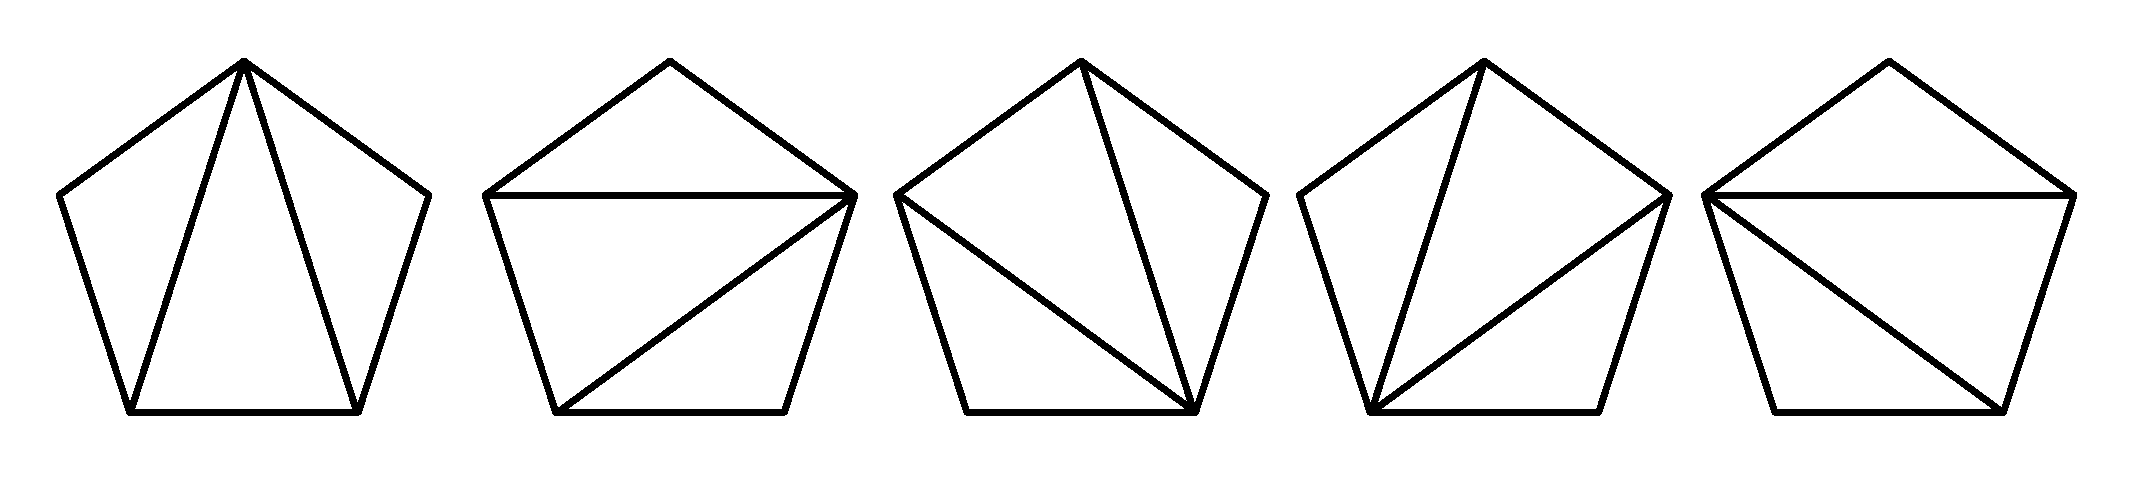
\includegraphics[width=0.7\textwidth]{images/title/5边形的划分方案.pdf}
		\caption{5边形的划分方案}
		\label{fig:5边形的划分方案}
	\end{figure}
	如下图\ref{fig:子问题归约}所示, $n$边形的顶点是$1,2,\cdots,n$. 顶点$i-1,i,\cdots,j$构成的凸多边形记作$A[i,j]$, 于是原始问题就是$A[2,n]$.
	\begin{figure}[H]
		\centering
		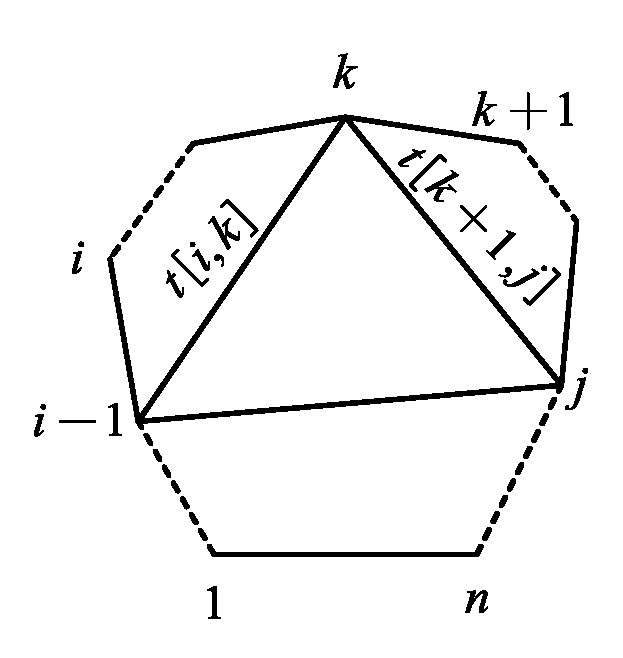
\includegraphics[width=0.25\textwidth]{images/title/子问题归约.pdf}
		\caption{子问题归约图}
		\label{fig:子问题归约}
	\end{figure}
	考虑子问题$A[i,j]$的划分, 假设它的所有划分方案中最小权值为$t[i,j]$. 从$i,i+1,\cdots,j-1$中任选顶点$k$, 它与底边$(i-1)j$构成一个三角形(图\ref{fig:子问题归约}中的三角形). 这个三角形将$A[i,j]$划分成两个凸多边形: $A[i,k]$和$A[k+1,j]$, 从而产生了两个子问题. 这两个凸多边形的划分方案的最小权值分别为$t[i,k]$和$t[k+1,j]$. 根据DP思想, $A[i,j]$相对于这个顶点$k$的划分方案的最小权值是
	$$
	t\left[ i,k \right] +t\left[ k+1,j \right] +d_{\left( i-1 \right) k}+d_{kj}+d_{\left( i-1 \right) j}
	$$
	其中$d_{\left( i-1 \right) k}+d_{kj}+d_{\left( i-1 \right) j}$是三角形$(i-1)kj$的周长, 于是得到递推关系
	$$
	t\left[ i,j \right] =\begin{cases}
		0,&		i=j\\
		\underset{i\le k\le j-1}{\text{min}}\left\{ t\left[ i,k \right] +t\left[ k+1,j \right] +d_{\left( i-1 \right) k}+d_{kj}+d_{\left( i-1 \right) j} \right\} ,&		i<j\\
	\end{cases}
	$$
	显然这个递推关系与矩阵链乘积算法的递推式十分相似, 可以通过标记函数来得到最小权值对应顶点$k$的位置, 并且类比矩阵链乘积算法, 可知该划分算法最坏情况下的时间复杂度为$O\left( n^3 \right)$.
\end{homeworkProblem}



\vspace{2cm}

至此, Chap 5的作业解答完毕.

\vspace{2cm}

\begin{figure}[H]  % 这里记得用[H]
	\centering
	
\includegraphics[width=0.7\linewidth]{images/title/ucas_logo 1.pdf}
	%\caption{ucas-logo}
	\label{fig:ucas-logo}
\end{figure}


% 引用文献
\bibliographystyle{unsrt}  % unsrt:根据引用顺序编号
\bibliography{refs}


\end{document}
